\section{Data Analysis}
\label{section:Data:DataAnalysis}

For any kind of prediction model to work, the underlying dataset needs some kind of recognisable pattern for
the model to learn.
In order to analyse the predictebilty of the data we checked for white noise, and if the time-series followed a random walk.

\subsection*{Theory}

\begin{figure}[H]
  \centering
  \caption{Syntetic data, noise and random values.}
  \label{fig:dataset:white_noise_random_wald}
  \begin{subfigure}[b]{0.4\textwidth}
    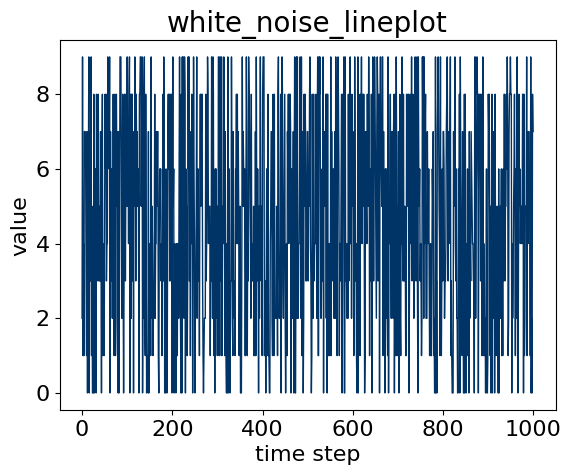
\includegraphics[width=\textwidth]{./figs/code_generated/data_exploration/white_noise_lineplot.png}
    \hfill
    \caption{White noise lineplot}
    \label{fig:dataset:white_noise}
  \end{subfigure}
  \begin{subfigure}[b]{0.4\textwidth}
    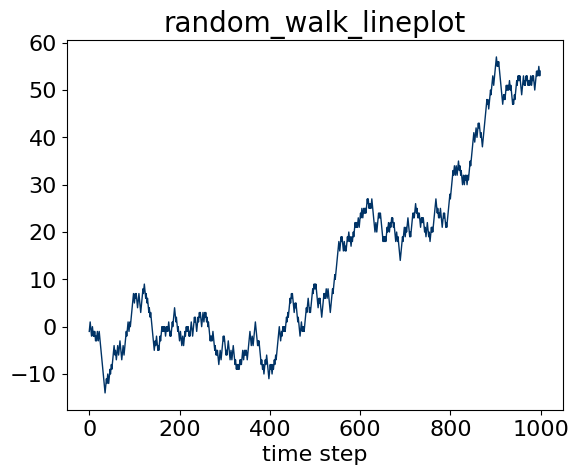
\includegraphics[width=\textwidth]{./figs/code_generated/data_exploration/random_walk_lineplot.png}
    \hfill
    \caption{A Random walk lineplot}
    \label{fig:dataset:random_walk}
  \end{subfigure}
\end{figure}



% TODO: [Move to B and T?]
White noise is just a random sample of numbers not following any pattern what so ever, as seen in
\Cref{fig:dataset:random_walk}.

A random walk is different from white noise, because the next value in the series is dependent on the previous value plus some noise.
\begin{equation}
  y_t+1 = y_t + r
  \label{eq:random_walk}
\end{equation}
where $r$ is some random number.
An example of a random walk graph is shown in \Cref{fig:dataset:random_walk}.

\Cref{fig:dataset:random_walk}.
\begin{figure}[H]
  \centering
  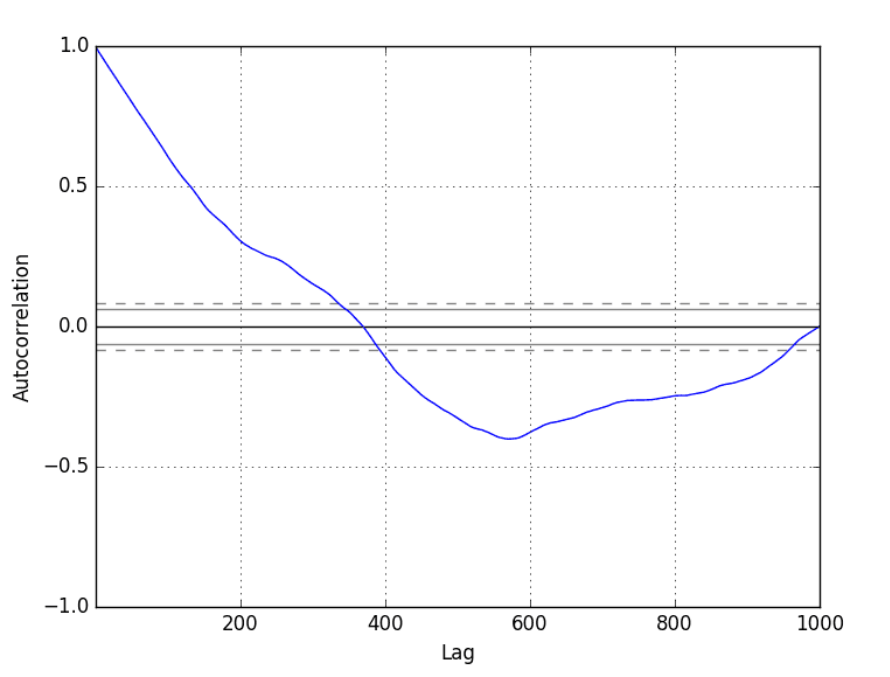
\includegraphics[width=0.5\textwidth]{./figs/illustrations/random_walk_autocorrelation.png}
  \hfill
  \caption{A Random walk autocorrelation}
  \label{fig:dataset:random_walk_autocorrelation}
\end{figure}

Since a random walk is highly dependable on previous values this will clearly show in an autocorrelation plot.
Which plots how much a series correlates with its previous values.
\Cref{fig:dataset:random_walk_autocorrelation} shows how a autocorrelation plot for the random walk in \Cref{fig:dataset:random_walk}.
It is a steadily decreasing trend which follows a linear pattern in the first 500 days.

One way to show if a series follows a random walk is to remove the temporal dependence by subtracting each value in the series by the previous value.
This will leave only the noise $r$ in Equation \Cref{eq:random_walk}.
If the series follows a random walk it will look a lot like the white noise shown in \Cref{fig:dataset:white_noise}.

Plotting the autocorrelation of the remainding noise $r$ in \Cref{fig:dataset:random_walk_noise_autocorrelation}
we can see the correlations are small, close to zero and below the 95\% (vertical dotted line) and the 99\% (vertical full line)
confidence levels.
\begin{figure}[H]
  \centering
  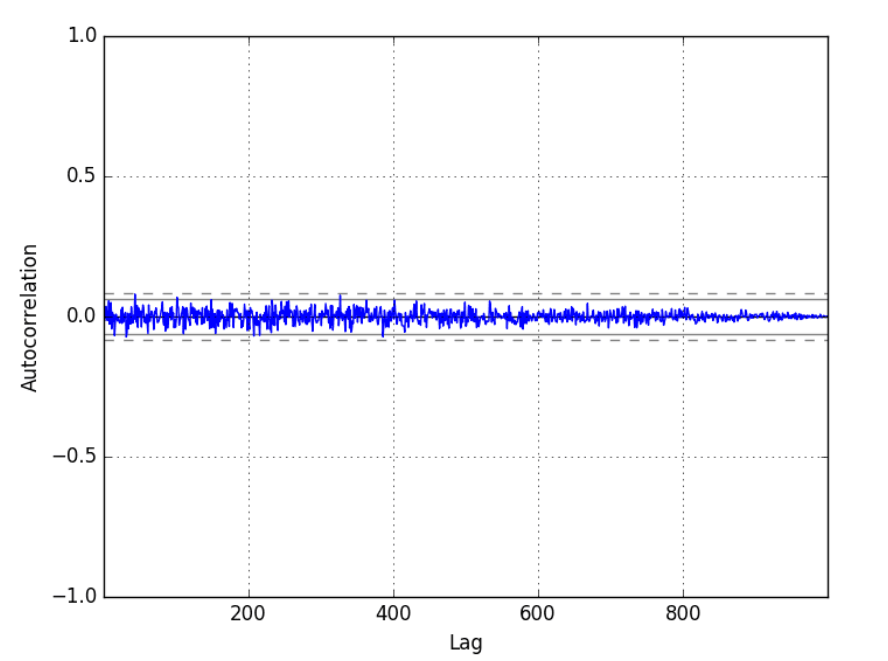
\includegraphics[width=0.5\textwidth]{./figs/illustrations/random_walk_noise_autocorrelation.png}
  \hfill
  \caption{A Random walk noise autocorrelatoin}
  \label{fig:dataset:random_walk_noise_autocorrelation}
\end{figure}
\begin{figure}[H]
  \centering
  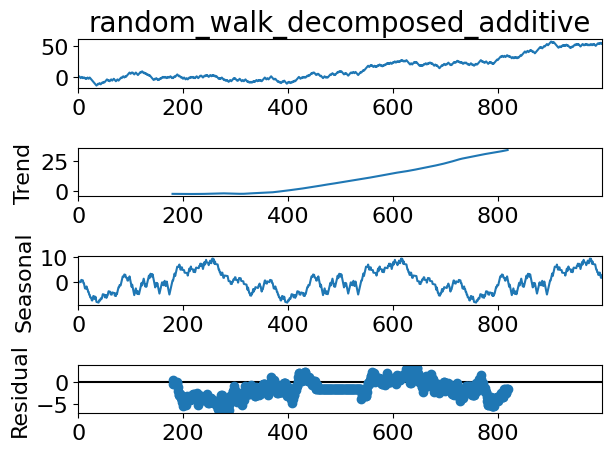
\includegraphics[width=0.5\textwidth]{./figs/code_generated/data_exploration/random_walk_decomposed_additive.png}
  \hfill
  \caption{A Random walk decomposed in Trend, Season, and rest}
  \label{fig:dataset:random_walk_decomposed}
\end{figure}


Characteristics of a random walk:
The time series shows a strong temporal dependence that decays linearly or in a similar pattern.
The time series is non-stationary and making it stationary shows no obviously learnable structure in the data.
The persistence model provides the best source of reliable predictions.

We chose a random sample of correlating categories to analyse,
and a set of highly seasonal categories.
Categories chosen was
%corr_categories cat: 2, 6, 9, 10, 11, 13, 20
%
%seasonal_categories_cat_name ["Vinterjakke",
%"Vintersko",
%"Langrennski",
%"Skisko",
%"Varmeovn",
%"Snøfreser",
%"Snøskuffe",]



By analysing a lag plot we can look for patterns in the data. A lag plot
show how much future values depend on past values.
% TODO: [Add lag plots].
The lag plot of.
% Write about dicky fuller test on dataset and decomposed resid.
% Write about how a lag plot of how a random walk looks like
% Write about how difference plot of random walk looks liks
% Write about lag plot and difference plot of our data 
% Check autocorrelation on random walk diff: https://machinelearningmastery.com/gentle-introduction-random-walk-times-series-forecasting-python/
\import{./tables/code_generated/data_exploration/}{dicky_fuller_test_residuals.tex}

\begin{figure}[H]
  \centering
  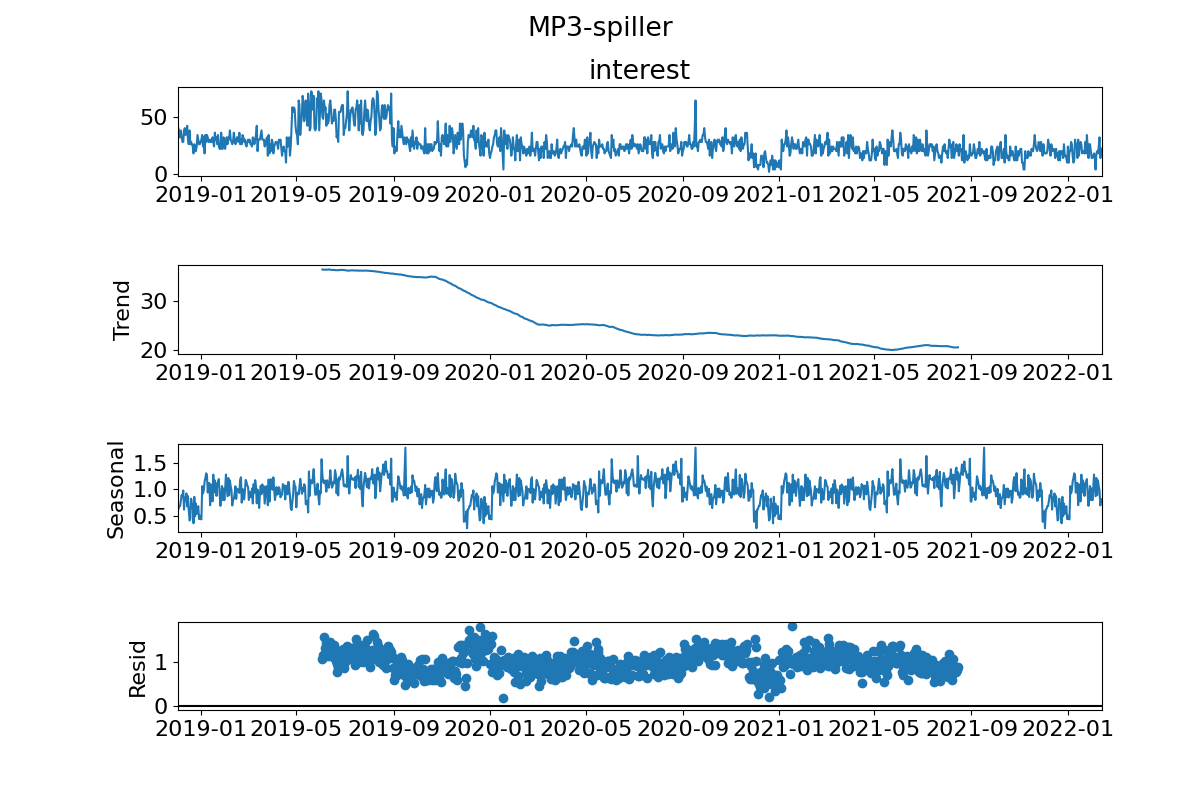
\includegraphics[width=0.9\textwidth]{./figs/code_generated/time-serie-MP3-spiller_decomposed.png}
  \hfill
  \caption{"MP3-spiller" decomposed}
  \label{fig:dataset:mp3-spiller-decomposed}
\end{figure}


